\documentclass[en,skiptoc]{../../../eplnotes}

\graphicspath{{img/}}
\usepackage{../../../eplunits}

\hypertitle{Cryptography}{8}{ELEC}{2760}
{Gaëtan Cassiers \and Benoît Legat \and Master students 2019}
{François--Xavier Standaert}

This document details the answers to the final quiz available on the course site.

\section*{Lecture 1}

\begin{enumerate}
    \item \textbf{Explain and define the concept of pseudorandom permutation \& secure encryption.}
    
    \begin{itemize}
        \item \textbf{Pseudorandom permutation}: a PRP is a one-to-one function which cannot be distinguished from a real random permutation: 
        $$ \Pr[Exp^{PRP}(n) = 1] - \frac{1}{2} \leq negl(n) $$
        \item \textbf{Secure Encryption}: An encryption is secure, if for every adversary $\mathcal{A}$ without unbounded power, we have 
        $$ \Pr[Exp^{CPA}_\mathcal{A}(n) = 1] - \frac{1}{2} \leq negl(n) $$
    \end{itemize}
    \vspace{5pt} \hrule
    \item \textbf{Compare the number of n-bit permutations and the number of n-bit keys. What does it imply regarding the indistinguishability of a block cipher from a random permutation?}
    
    \begin{itemize}
    \item number of n-bit keys = $2^n$
    \item number of n-bit permutations = $(2^n) !$
    \end{itemize}
    As $2^n \ll (2^n) !$, we can deduce that a block cipher is distinguishable from a random permutation, only if we have unbounded power.
\end{enumerate}

\section*{Lecture 2}

\begin{enumerate}
  
    \item \textbf{Explain the reduction from secure encryption to 1-bit pseudorandom generator.}
    
    We can build a 1PRG with 1 bit expansion to support secure encryption: 
    $$ x_{i+1} = g^{x_i} \text{ mod } p, \text{output 1 if } x_{i+1} < \frac{p-1}{2} $$
    \vspace{5pt} \hrule
    
    \item \textbf{Express $\mathbf{Adv}^{\mathrm{nPRG}}_\mathrm{A}$ in function of $\mathbf{Adv}^{\mathrm{1PRG}}_\mathrm{A}$ if the only possible attack considered by the adversary A is to target all the nPRG blocks independently.}       
    As the adversary does not consider slide attack, we can deduce its only option would be attacking each 1PRG independently. If an attack of one of the 1PRG success then he can break the nPRG. So we have:
    \begin{align*}
        \mathbf{Adv}^{\mathrm{nPRG}}_\mathrm{A} &= 1-(1- \mathbf{Adv}^{\mathrm{1PRG}}_\mathrm{A})^n\\
        &\approx n\cdot\mathbf{Adv}^{\mathrm{1PRG}}_\mathrm{A} \text{\qquad (if $\mathbf{Adv}^{\mathrm{1PRG}}_\mathrm{A}$ is small)}
    \end{align*}
    
    \vspace{5pt} \hrule
    
    \item \textbf{Express $\mathbf{Adv}^{\mathrm{CBC}}_\mathrm{A}$ in function of $\mathbf{Adv}^{\mathrm{1PRP}}_\mathrm{A}$ if the only possible attack considered by the adversary is a collision attack. Can you say CBC is a secure encryption mode? Why?}
    
    
    Assuming each block is independent, the probability of a collision (ie two outputs of the
    PRP are the same) is approximately $q^2/2^{n+1}$ (birthday attack), for $q$ blocks.
    Such a collision allows to recover the XOR of two plaintext blocks.
    
    Since this attack has a success probability that is a negligible function of $n$
    (when $q$ is a polynomial function of $n$), it is not a threat to the security of the
    CBC mode.   

    \vspace{5pt} \hrule
    
    \item \textbf{Express $\mathbf{Adv}^{\mathrm{PRP}}_\mathrm{A}$ in function of $\mathbf{Adv}^{\mathrm{1PRF}}_\mathrm{A}$ based on Luby \& Rackoff’s theorem. Is the bound tight (i.e. is there an attack matching this bound)?}
    
    For an attack whith $q$ choosen plaintexts and a PRF over $n$ bits (thus PRP over $2n$ bits):
    $$\mathbf{Adv}^{\mathrm{PRP}}_\mathrm{A} \le 3\  \mathbf{Adv}^{\mathrm{1PRF}}_\mathrm{A} + \frac{q^2}{2^{n+1}}$$
    
    This bound is tight: the part $3\  \mathbf{Adv}^{\mathrm{1PRF}}_\mathrm{A}$ corresponds to the independent attacks against
    the 3 PRFs.
    The part $\frac{q^2}{2^{n+1}}$ corresponds to a simple chosen plaintext collision attack:
    let the plaintexts $(x_i, y)_{i=1,...,q}$ be encrypted (the second part $y$ of the plaintext is constant).
    The input of the first PRF $f_1$ are thus constant. If there is a collision on the second PRF,
    ie $f_2(x_i \oplus f_1(y)) = f_2(x_j \oplus f_1(y))$ for some $i \neq j$, then the first halves of the
    outputs are the same, and the XOR of the second halves of the outputs is equal to the XOR of the
    second halves of the inputs.

    The probability that such a collision on the output occurs for a Luby-Rackoff PRP is thus $q^2/2^{n+1}$
    (probability of birthday style collision on the input of $f_2$ for random $x_i$). For a true RP the collision
    probability is much lower (but hard to estimate, for a RF it would be $q^2/2^{2n+1}$).

    \vspace{5pt} \hrule
    
    \item \textbf{Explain the concept of Time-Memory Tradeoff in the context of exhaustive key search. How can you choose its parameters to efficiently deal with chains merging?}
    
    In brute force attacks, there are $N=2^n$ solutions. This solution can be found whether doing $T$ operations at the attack time, or by pre-computing M values and storing them in a look-up table. It is also possible to do a time-memory trade-off, by using both approaches, as long as $M \cdot T \geq N$.
    
    In the article L2\_R1, it is proposed a trade-off between $t$ (\# columns) and $m$ (\# rows) such that:
    
    \begin{figure}[h!]
        \centering
        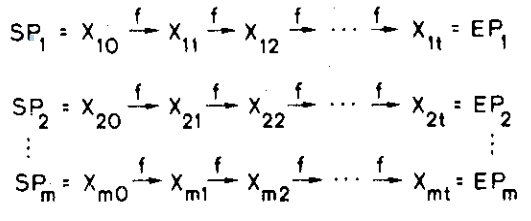
\includegraphics[width=7cm]{TM_tradeoff_approach.png}
        \caption{time memory trade-off}
        \label{fig:my_label}
    \end{figure}
    
    In this configuration, $M=mt$, $T=t^2$.We can set $m \cdot t^2 = N$, such that $t=m=N^{1/3}$ and the previous condition is satisfied. 
    
    Using this strategy $M=T=N^{2/3}$, which is significantly better than the original $M=N$ for using only memory or $T=N$ for using just time.
    
    We can expand the parameters $m$ and $t$ up to $mt^2 = 2^n$.
    \vspace{5pt} \hrule
    
    \item \textbf{Describe an attack against 2DES in less than $2^{57}$ time. How to avoid it?}
    
    We will use the meet-in-the-middle attack. First we must acquire $y_1 = DES_{k_1}(x_1)$ and attack it. The complexity of this attack would be $2^{56}$. Then we would do the same to get $k_2$, leading to a complexity of $2 \times 2^{56} = 2^{57}$. We can avoid it by modifying the encryption with 3DES by $c = E_{k_1}(D_{k_2}(E_{k_1}(m)))$. \href{https://www.nku.edu/~christensen/3DES.pdf}{Explained here}.
    \vspace{5pt} \hrule
    
    \item \textbf{Explain how to attack one DES round (simplified to 32-bit round keys and 4-bit bijective S-boxes). Give the attack complexity. How would this complexity approximately scale (in the worst-case) if two DES round have to be attacked?}
    
     We can build an efficient attack to find the 32-bit key. First we obtain $f_k(R_0) = R_1 \oplus L_0$. Then, as the function is composed of 8 SBOX, taking 4bits keys, we can do exhaustive key search on those small key size.\newline
     \textbf{Attack complexity }: $8 \cdot 2^4 $.

    For two rounds, since we have a Feistel network, the attack to recover the second subkey is the same, and the attack
    to recover the first subkey is almost the same (there is a first XOR needed to find the output of the DES PRF).

    The complexity of these attack have the same order of magnitude, the time required is doubled.

    \vspace{5pt} \hrule
    
    \item \textbf{Explain the concept of slide attack. Is a block cipher susceptible to this attack a PRP?} 
    
     The goal is here to find the $BC_k(m)$ of the first round to use the previous algorithm to find $k$. First we take a lot of pairs $(x_0, x_1)$ assuming $x_1 = BC^{oneRound}_k(x_0)$ (on one round of BC of course), and compute the key that verifies this relation. To confirm if the assumption was correct, we simply evaluate $y_i = BC_k(x_i)$, and check if $y_1 = BC^{oneRound}_k(y_0)$. If it is true, we have found the key. We want to know how many pairs of plaintexts we have to compute in order to have a collision in the ciphertexts. By the birthday paradox, we need $2^{n/2}$ pairs in general to find a collision with probability 40\%, leading to a time complexity of $8 \cdot 2^4 \cdot 2^{n/2}$. But it is even less for a Feistel cipher since half of the ciphertext is independent of the key. We thus have to find $2^{n/4}$ pairs for a Feistel cipher, leading to a time complexity of $8 \cdot 2^4 \cdot 2^{n/4}$.
     
     In the strict sense, since the complexity of the slide attack
     is exponential ($2^{n/2}$), this attack does not allow to build a distinguisher that breaks the PRP property.
     However, this attack reduces significantly the security since usually the best attack against a block cipher is
expected to be $\mathcal{O}(2^n)$.
\end{enumerate}

\section*{Lecture 3}
\begin{enumerate}
    \item \textbf{Give a proof of the piling-up lemma.} 
    
    Pilling-up lemma:
    \[\Pr[X_1 \oplus ... \oplus X_n = 0] =
    \frac{1}{2} + 2^{n-1} \prod_{i=1}^n \left(\Pr[X_i=0] - \frac{1}{2}\right)\]

    For $n=1$, this is trivially true. Let $Y_n = X_1 \oplus ... \oplus X_{n-1}$.
    By induction,
    \[\Pr[Y_n = 0] = \frac{1}{2} + 2^{n-2}\prod_{i=1}^{n-1} \left(\Pr[X_i=0] - \frac{1}{2}\right).\]
    Then,
    \begin{align*}
        \Pr[Y_n \oplus X_n = 0] &= \Pr[Y_n = 0, X_n = 0] + \Pr[Y_n = 1, X_n = 1] \\
                            &= \frac{1}{2} + 2\left(\Pr[X_n = 0] - \frac{1}{2}\right)
        \left(\Pr[Y_n = 0] - \frac{1}{2}\right) \\
        &= \frac{1}{2} + 2^{n-1}\prod_{i=1}^n \left(\Pr[X_i = 0] - \frac{1}{2}\right).
    \end{align*}
    
    \vspace{5pt} \hrule
    
    \item \textbf{Explain why a linear permutation cannot be a good block cipher.}  
    
    A linear permutation can be solved using a system of linear equation, and linear equations can be easily solved. This is why it can not be a good block cipher.
    
    Let $(x_1, x_2, ..., x_n)$ a basis of $\{0,1\}^n$. If the output of the linear permutation
    is known for all the elements of the basis: $y_i = F(x_i)$, $F(x)$ is known for any $x$:
    let $x = \sum_{i=1}^n a_i x_i$, then $F(x) = \sum_{i=1}^n a_i y_i$.
    
    \vspace{5pt} \hrule
    
    \item \textbf{Explain the concept of linear cryptanalysis and give its data complexity.}  
    
    Linear  cryptanalysis  tries  to  take  advantage  of  high  probability  occurrences  of  linear expressions involving plaintext bits, "ciphertext" bits,  and  subkey  bits.
    
    This linearity can be exploited by analysing the probability of any linear operation involving input and outputs of a system. In our studies, we have chosen to analyse the linearity involving the input bits $a_i\cdot x_i$ and the output bits $b_{i+1}\cdot x_{i+1}$ of the $i^{th}$ Sbox through the function
    
    $$ a_i\cdot x_i \oplus b_{i+1}\cdot x_{i+1}$$
    
    which should equals 0 with probability $1/2$ if no linearity was observed.
    
    \textbf{Data Complexity: } $N \propto \frac{1}{\epsilon^2}$ where $\epsilon$ is the bias
    \vspace{5pt} \hrule
    
    \item \textbf{Why does the AES block cipher start/end with a key addition?}  
    
    Any  layer  after  the  last  key  addition  in  the  cipher  (or  before  the  first  in  the context of known-plaintext attacks) can be simply peeled off without knowledge of the key and therefore does not contribute to the security of the cipher. In other words, without this, operations not between key additions are useless from a security view point.
    
    The operations of AES that are not key addition are public bijections.
    If AES were $A(B_k(C(\cdot)))$, any attack against $B_k$ could
    easily be turned into an attack against AES by applying $A$, $C$
    or their inverses where needed.
    The operations $A$ and $C$ bring thus no security benefit.
    
    \vspace{5pt} \hrule
    
    \item \textbf{Why does the AES block cipher have no MixColumns operation in its last round?}  
    
    It does not change the security: since $MC$ is linear,
    $K_n \oplus MC(x) = MC(MC^{-1}(K_n) \oplus x)$.
    Then the outer $MC$ can be removed by any attacker.

    \vspace{5pt} \hrule
    
    \item \textbf{Is $AES_k(AES_k(x))$ stronger than $AES_k(x)$ from the linear cryptanalysis point-of-view?}  
    
    No. The LCB decreases exponentially with the number of rounds, but the ELB does not due to the
    linear hull effect.
    Since the maximum LCB of AES reduced to four rounds is $2^{-100}$, it is expected that the ELB for
    full AES (10 rounds) is close to a minimum LB possible for a 128 bits permutation.
    
    See L3\_R2, "Experimenting Linear Cryptanalysis" section 2.3.
    
    \vspace{5pt} \hrule
    
    \item \textbf{Explain the wide-trail strategy, its application to the AES and the bounds that can be obtained for 4 AES rounds against linear criptanalysis.  What are the main (theoretical) limitations of this strategy (and how to mitigate them)?}  
    
    Wide trail strategy: have low biases in reasonably-sized S-Boxes, and use diffusion layers to have
    many active S-Boxes for each characteristic. For AES, there are at least 25 active S-Boxes active for
    any 4 round characteristic. The ELB of and S-Box is $\le 2^{-4}$, thus the LCB of any 4-round characteristic
    is at most $2^{-100}$. (Thus an attack has a data complexity of $2^{200}$.)

    This strategy is limited by presence of multiple characteritics for the same input-output mask:
    the linear hull. The total ELB is thus the sum of the LCB for all the characteristics of the
    linear hull, and not the maximum LCB. The LCB is also estimated by assuming independence between biases.

    Increasing the number of round is a way to reduce the LB up to some point (usually when the
    LB is close to the minimum possible for a permutation: $2^{-n}$).
    
    To define it properly, we need some definitions:
    
    Linear bias between input $X$ masked by $a$ and output $F_k(X)$ masked by $b$: 
    $$ LB(a,b,k) = \Pr[a\cdot X = b \cdot F_k(X)] - \frac{1}{2}$$
    
    Expected linear bias of $F(X)$ when using key $k$:
    $$ ELB(a,b,k) = E_{X,k}[LB(a,b,k)]$$
    
    
    One-round characteristic for round $i$, giving the input/output masks to be applied for the LB calculation:
    $$<a_i, b_i>$$
    
    And R-round characteristic for rounds $1,\dots,R$:
    $$\Omega = <a_1,\dots, a_R, a_{R+1}>$$
    
    If we assume a Markov cipher (linear and differential probabilities of different rounds independent of each other), the linear characteristic bias of R rounds is:
    
    $$LCB(\Omega, \tilde{K}) = 2^{R-1} \cdot \prod^{R}_{i=1}LB(a^i, a^{i+1}, k^i) $$
    
    The wide trail strategy \textit{assumes} key equivalence, e.g.:
    $$ELB(a,b,k) \approx LCB(\tilde{\Omega}_{best})$$
    
    And it requires that $LCB(\tilde{\Omega}_{best})$ is as small as possible. To achieve it, the Sboxes must have low linearity and there must be as Sboxes as possible in each path.
    
    The weaknesses of this strategy are mainly associated with the assumptions made. First of all, all the subkeys are derived from a unique key, and therefore they are not independent from one another.Moreover the key equivalence assumption is not totally true
    

    
    \vspace{5pt} \hrule
    
    \item \textbf{Why are the various representations of the AES components relevant from an implementation point-of-view and from a physical security point-of-view?} 
    
    Representations:
    \begin{itemize}
        \item Elements of $GF(8)$, $GF(32)$: mathematical properties useful for proofs
            (eg. MDS property of MC), and map to efficient representation on HW, and 
            particularly on general purpose CPUs (bytes, and words for 32-bits machines).
        \item S-Box: Lookup table (efficiency) or affine transformation of multiplicative
            inverse in GF(8) (structure, no backdoor) or logic equations (bitslicing,
            masked implementations).
    \end{itemize}    
    
    \end{enumerate}

\section*{Lecture 4}
\begin{enumerate}
    \item \textbf{What is the activity factor of a block cipher implementation (after some rounds)?}  
    
    The activity factor is the number of bit switches. It is also defined as the fraction of time that a power node is consuming power.
    
    Reference \href{https://books.google.be/books?id=yb99g5G7FS4C&pg=PA136&lpg=PA136&dq=cryptography+\%22activity+factor\%22&source=bl&ots=qBtsSWgl5Z&sig=ACfU3U1faD9lVj3G3EACeV12p7dQEhsYNg&hl=en&sa=X&ved=2ahUKEwjumqnB9-niAhUCr6QKHUdNAp4Q6AEwAHoECCMQAQ#v=onepage&q=cryptography\%20\%22activity\%20factor\%22&f=false}{here} or \href{https://www.esat.kuleuven.be/cosic/publications/thesis-124.pdf}{here}.
    
    After some rounds the value should be uncorrelated with the input,
    and all the values are equiprobable for random inputs (since each intermediate value is a permutation
    of the input for a fixed key). The activity factor is thus 0.5.
    The sum of two bit values (that should be uncorrelated between each other) is thus equiprobably 0 or 1.
    
    \vspace{5pt} \hrule
    
    \item \textbf{Describe the structure of an FPGA and detail an exemplary slice with 4-bit LUTs.}
    
    FPGA's are formed by several blocks whose I/Os can be routed between each others'. The main blocks of those components are: I/O buffers, routing block, embedded block (memory, multiplier, etc) and logic blocks (LB). LB are the ones responsible for performing the binary operations, which is done through look-up table (LUT) and arithmetic and logic units (ALU). They also may have sequential logic elements, such as flip-flops. 
    
    For example: 2 4-bit LUT, 1 MUX, 2 flip-flops.
    
    \vspace{5pt} \hrule
    
    \item \textbf{Explain the difference between the minimum memory cost and the concrete implementation cost of an S-box and discuss its relevance in a performance evaluation.}
    
    For building an Sbox, the minimum memory cost is the number of memory bits needed for this task according to a certain Sbox structure. In the course, two Sbox structures have been studied:
    
    \begin{figure}[h!]
        \centering
        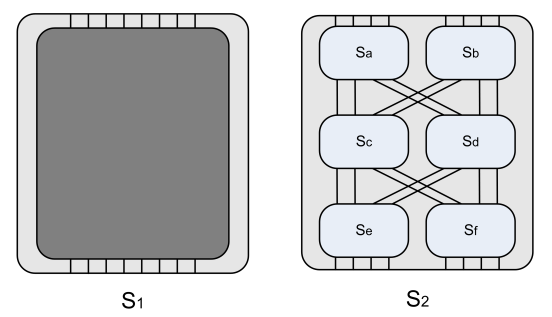
\includegraphics[width=8cm]{sboxes_implementation_architectures.png}
        \caption{Internal Sbox architectures}
    \end{figure}
    
    For building S1 as a table we need $8 \cdot 2^8=2048$ bits of memory, while for building S2 we need $6 \cdot ( 4 \cdot 2^4) = 384$ bits.
    
    In order to build Sboxes with FPGA we need to use LBs, though. We consider now to different LB architectures for making it:
    
    \begin{figure}[h!]
        \centering
        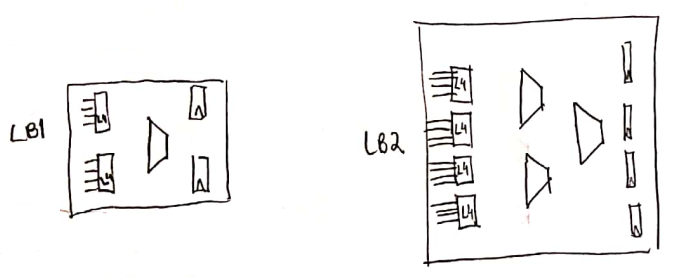
\includegraphics[width=10cm]{LB_schemes.png}
        \caption{LB architectures}
    \end{figure}
    
    The arrangements of those LBs for achieving the corresponding to one 8 to 1 multiplexer were detailed in class, but the results are summarised in the table:
    
    \begin{table}[h!]
    \centering
    \begin{tabular}{|l|l|l|}
    \hline
    multiplexer & \# LB1                  & \# LB2        \\ \hline
    M5          & $1\cdot LB1$            & $1 \cdot LB2$ \\ \hline
    M7          & $4M5+LB1 = 5\cdot LB1$  & $1 \cdot LB2$ \\ \hline
    M8          & $2M7+LB1 = 11\cdot LB1$ & $1 \cdot LB2$ \\ \hline
    \end{tabular}
    \end{table}

    One can now analyse the cost (number of LBs needed) of implementing those Sboxes in different architectures:
    
    \begin{table}[h!]
    \centering
    \begin{tabular}{|l|l|l|}
    \hline
       & LB1                                   & LB2                            \\ \hline
    S1 & $8\cdot M8=8\cdot 11 \cdot LB1$       & $8\cdot M8=8\cdot LB2$         \\ \hline
    S2 & $6 \cdot (2 \cdot LB1)= 12 \cdot LB1$ & $6 \cdot (LB2)= 6 \cdot LB2$ \\ \hline
    \end{tabular}
    \end{table}    
    
    The minimum memory cost of an S-Box is the total size of memory used by the implementation
    that has LUTs of optimal sizes, that are optimally routed.
    In actual FPGAs, the LUTs may not have the optimal size so the implementation cost may be higher.
    This can lead to a larger number of slices used in such an FPGA.
    
    \vspace{5pt} \hrule
    
    \item \textbf{For any exemplary block cipher architecture (serial, parallel, with or without pipeline,...), estimate its cost, latency and throughput under reasonable assumptions. Why are such handmade prelimiary estimations useful for a designer/implementer?}
    
    \vspace{5pt} \hrule
    
    \item \textbf{Can you exploit pipelining to implement the CBC mode of operation? Why?}
    
    For encryption, CBC is a serial mode: the ciphertext of the previous block must be known to begin the
    encryption of the following block, since $c_i = BC_k(c_{i-1} \oplus p_i)$.
    Pipelining being a form of parallel computation, it can not be used with CBC, except if
    multiple independent streams of data have to be encrypted.

    For decryption, there is no such dependence (since $p_i = BC^{-1}_k(c_i) \oplus c_{i-1}$),
    so pipelining can be exploited.
    
\end{enumerate}

\section*{Lecture 5}
\begin{enumerate}
    \item \textbf{ In order to minimize the energy consumption of an implementation, would you select a more serial (e.g. 8-bit) or a more parallel (e.g. 32-bit) architecture?}
    
    For example, if the 32-bit architecture consumes four times more current than the 8-bit architecture under the same conditions (same operating frequency and same supply voltage), then if one 32-bit operation translates into more than four 8-bit operations, the 32-bit architecture is more energy efficient.

    With SW implementation, on 32 bits architectures, T tables lead to a cost of around 2 instructions
    per byte and ber round (of which 1 memory lookup)
    for AES.
    (Also more 16 times memory used, which increases memory power consumption.)
    On 8 bit architecture, 2 mem lookup, order of 5 other instructions per byte and per round.

    There is thus no clear advantage for one or the other implementation here.
     
    \vspace{5pt} \hrule

    \item \textbf{Discuss the interest of moving an S-box in RAM in a software block cipher implementation (under reasonable assumptions on the elementary operation’s cost).}
    
    The S-box is usually stored initially in ROM because it is not volatile but it takes 3 cycles to read, while the RAM takes only 2 cycles but it is volatile. It makes sense to move it to the SRAM if the gain is worth all the cycles needed to move it (1280 cycles, moving 256 bytes with each taking 3 cycles to read from ROM and 2 cycles to write on RAM).
    
    $3N>2N+1280$, meaning that it is worth it to move it to RAM if at least 1280 S-boxes are going to be computed, around 8 AES encryptions.
    
    \vspace{5pt} \hrule

    \item \textbf{ Assuming a 64-bit ALU, what is the maximum number of gates per output bit which makes a bitslice implementation of an 8-bit S-box interesting from the performance point of view (under reasonable assumptions on the elementary operation’s cost)?}
    
    If an 8-bit S-box takes N gates per output bit and 1 cycle per gate to be computed with an ALU and only 1 lookup table, 5 cycles per lookup table.
    
    $$
    \frac{N\cdot8}{64}<5
    $$
    The maximum number of gates is thus 40.
    
    \vspace{5pt} \hrule

    \item \textbf{Estimate the implementation cost of the xtime function implemented as a table (in cycles and memory) and as Boolean operations (in cycles and code size).}
    
    The $xtime(a)$ operation is a multiplication of $a$ by 2 in GF(8), which is performed as follows:
    
    $$
    \mathrm{xtime}(a) =  \begin{cases}
                (a_6,...,a_0,0) \text{, if } a_7=0 \\
                (a_6,...,a_0,0) \oplus (0,0,0,1,1,0,1,1) \text{, if } a_7=1  
                \end{cases}
    $$
    
    Where $m(x) = (0,0,0,1,1,0,1,1) = x^4 +x^3 + x +1$.
    
    For implementing it with Boolean operations, one can do a shift and conditionally an addition. When it comes to low level coding, some assembly languages allow to do both operations at once, in one elementary operation of the language. This is important to reduce data-dependency of the power consumption, which can be exploited in side channel attacks. Moreover, this operation does not require more than one register in the processor. It needs around 6 cycles
    
    For implementing it in memory, there must be $2^8$ possible entries addressing one byte each. it gives a total of $2^8 \cdot 8$ bits consumed in memory, besides the access time that may be of 1 clock cycle if it is stored in RAM or about 3 if it is stored in ROM.
    
    \vspace{5pt} \hrule

    \item \textbf{Detail the T-table technique for the combined implementation of the AES S-box and MixColumns layers. Estimate its cycle count and memory cost?}
    
    The idea here is to perform both Mix--Columns and Sbox transformation in 4 memory accesses and three additions of vectors, for 32-bit architecture.
    
    \[
    \begin{pmatrix}y_0\\ y_1\\ y_2\\ y_3\end{pmatrix}
        \begin{pmatrix}
            02 & 03 & 01 & 01 \\
            01 & 02 & 03 & 01 \\
            01 & 01 & 02 & 03 \\
            03 & 01 & 01 & 02 
        \end{pmatrix}
    \begin{pmatrix}x_0\\ x_1\\ x_2\\ x_3\end{pmatrix}
        =
    \begin{pmatrix}02\\ 01\\ 01\\ 03\end{pmatrix} SB(x_0) +
    \begin{pmatrix}03\\ 02\\ 01\\ 01\end{pmatrix} SB(x_1) + ...
        = T_0(x_0) + T_1(x1) + ...
    \]
    where $T_i$ tables are 4 tables with 256 entries of 32 bits.
    The memory cost is thus \SI{4}{kiB}, and the cycle count
    is 16 memory accesses plus 12 XOR for the complete layer of SB + MC of
    one round.
    
    If it was implemented in 8-bit, each T would have to be subdivided in 4, leading to a final 15 8-bit sums.
    
\end{enumerate}

\section*{Lecture 6}
\begin{enumerate}
    \item \textbf{Explain the concept of a Differential Power Analysis (e.g. against the DES or AES). Are there weak keys in this context (i.e. keys that are easier to recover than others)?}
    \vspace{5pt} \hrule
    
    \item \textbf{Explain the concept of asymptotic equivalence between the CPA and template distinguishers. Under which conditions is this equivalence observed in practice?}
    
    Here is a good article co-produced by the teacher himself: \\ \url{https://perso.uclouvain.be/fstandae/PUBLIS/92.pdf}.
    
    \vspace{5pt} \hrule

    \item \textbf{For an exemplary block cipher architecture (in hardware or software) and using the abstractions of Lectures 4 and 5, estimate the security level of an implementation based its "algorithmic noise" and given a "physical noise" level. What can you conclude from such
estimations regarding the use of noise as an implementation security parameter?}

    Let $L$ the leakage, $M_k$ the modelled leakage, $N_a$ the algorithmic noise and
    $N_p$ the physical noise. We have $L = M_k + N_a + N_p$. We compute
    $\rho(L, M_k) = \rho(L, M_k+N_a), \rho(M_k+N_a, M_k)$, where $\rho{M_k+N_a, M_k} = \sqrt{m/n}$,
    where $n$ is the architecture number of bits and $m$ is the number of bits predicted by the model.
    Since the data complexity $N$ is proportional to $1/\rho(L, M_k)^2$
    (we try to distinguish between the correlation for the correct key $k$ and the
    distribution for a wrong key $k'$, assuming $\rho(L, M_{k'}) = 0$), it is proportional to $n$ (for fixed $m$),
    which means that algorithmic noise is not a good security parameter (complexity for the adversary
    is only proportional and not exponential in the security parameter $n$).
    
    Assuming independent
    $M_k+N_a$ and $N_p$, let $\sigma_a^2$ the variance of $M_k+N_a$ and $\sigma_p^2$ the
    variance of $N_p$, we have $\rho(L, M_k+N_a) = \sigma_a / \sigma_p = \sqrt{SNR_p}$,
    where $SNR_p$ is the pysical SNR. We have thus $N \propto SNR_p$, which means that
    physical noise is not a good security parameter.

\end{enumerate}

\section*{Lecture 7}

\begin{enumerate}
  
    \item \textbf{ Explain the concept of masking. Why can we say that masking amplifies the noise in a side-channel attack? What are the main assumptions for masking to deliver security?}
    
    Here is a useful link to understand where the security comes from: \url{https://orbilu.uni.lu/bitstream/10993/10582/1/splimaskanalysis.pdf}
    
    \vspace{5pt} \hrule
    
    \item \textbf{For simple (e.g. encoding, addition or multiplication) gadgets, exhibit probing attacks and discuss whether the probing security is optimal or not. Same question if the implementation exhibits physical defaults such as distance-based leakages, couplings.}
    
    Maybe slide 6 for probing attacks and slide 10 for the physical defaults?
    
    \vspace{5pt} \hrule
    
    \item \textbf{For simple encoding and leakage functions, plot the leakage distributions for simple leakage functions and motivate the definition of statistical security order based on them.}
    
    \vspace{5pt} \hrule

    \item \textbf{Explain why an information theoretic metric (such as the mutual information) is needed to capture the security of a masked implementation (and why the correlation coefficient is not enough in this case). Discuss the contexts in which the MI and correlation metrics are equivalent and their relevance to security evaluations.}
    
    The correlation coefficient is not enough since it uses only the first order moment of the leakage distribution, which the mean of the distribution. It thus prevents this method to recover the information if it is masked. The Mutual Information uses higher order moments of the distribution in order to find the variable even if it masked.
    
    Correlation and MI metrics are equivalent in a system that is nos using masking, since they can both break the information in this case.
    
    \vspace{5pt} \hrule

    \item \textbf{For simple combinations of addition and multiplication gadgets (such as the multiplication chain for the AES S-box), estimate the security level of a masked implementation considering different noise levels (captured by an MI curve), number of shares, and more or less powerful adversaries (i.e. exploiting one tuple of leakage samples, all leakage samples, averaging, with or without physical defaults,\dots). Discuss the relative importance of these different contexts and parameters on the implementation security level.}
    
    
\end{enumerate}

\section*{Lecture 8}

\begin{enumerate}

    \item \textbf{Describe different solutions to insert faults in a block cipher implementation, ranging
from cheap to expensive. How would you evaluate the usefulness of a fault from the the
adversary’s viewpoint? Discuss the tradeoff between a fault’s usefulness and practicality}
   \begin{itemize}
       \item Cheap: \begin{itemize}
           \item Reduce supply voltage
           \item Increase clock frequency
           \item Glitches
           \item Increase temperature
       \end{itemize}
       \item Intermediate cost: EM perturbation or Light/lasers
       \item Expensive cost: particles (cyclotron)
   \end{itemize}
   Usefulness of a fault is evaluated by 3 criterion:
   \begin{itemize}
       \item Number of fault needed to recover the key
       \item Precision of the fault required (very precise bit/byte, any byte,...) 
       \item Difficulty of the fault (\textit{random byte} is easier than \textit{toggle bit} which is easier than \textit{set bit})
   \end{itemize}
   All the tradeoff is between these 3 criterions: very precise fault could help recover the key very fast (e.g set a bit to 0 and check if there is a change in the cipher allows to directly recover a bit of the key) but are hard to put in place.
    \vspace{5pt} \hrule
    
    \item \textbf{Describe a fault attack against the AES targeting (i) the last round S-box with a toggle
bit model and (ii) the MixColumns operation between rounds 8 and 9 with a random byte
error model. Discuss the efficiency vs. feasibility tradeoff of these attacks.}
   
    \vspace{5pt} \hrule
    
        \item \textbf{ Evaluate the (time and data) complexity of a fault attack by reasoning on the mutual
information provided by simple fault models (i.e. by counting key candidates).
}
   
    \vspace{5pt} \hrule
    
    \item \textbf{Propose countermeasures against fault attacks. Discuss their assumptions.}
    There exist two types of countermeasures: 
   \begin{itemize}
       \item Time redundancy: \textit{e.g: encrypt twice, encrypt and decrypt to check no error occured.}
       \item Data redundancy: \textit{e.g: parity check or error correcting code on the data to check no corruption.}
   \end{itemize}
   These countermeasures assumes that adversary could not insert very precise faults (e.g twice the exact same fault to avoid double encryption check) and that the comparison actually takes place. 
    
\end{enumerate}




\end{document}
